\chapter{COMPARING THE COUNTRIES}
\label{sec:fourth}


In this chapter, we want to compare four countries: Italy, Spain, Sweden and Norway. 
That is two countries from the Mediterranean and two countries from Scandinavia.
The availability of the data in the Human Mortality database varies for these countries.
The mortality series are as follow: in Norway we have data for 1846-2014, Sweden 1751-2017, Italy 1872-2014 and Spain 1908-2016.
To have uniform data sets for the four countries we choose to look at developments from the calendar year 1910 (since mortality data for Spain are available only from the year 1908) to the calendar year 2014 (since Norway and Italy have mortality data until only 2014).
The ages varies between 0 and 110 years.

\section{Period data}

\subsection{Period Mortality}

Over the last century, countries across the Mediterranean and Scandinavia have seen a lot of variation in mortality.
In this section we will see how the period mortality has change during the years.
The visualization from figure \ref{fig:Period mortalityRate 1920} to figure \ref{fig:Period mortalityRate 2014}  shows the evolution of the period mortality rates in Italy, Spain, Sweden and Norway during the years 1920, 1950, 1980 and 2014. 
For all four countries, we can observe that the  mortality rate is generally very high from  birth but decrease drastically and attain a minimum level around age 10. 
During the adolescence  until around the age of 30, we can observe a stagnation of the mortality. 
From age 35 years and beyond, we observe an exponential increase of mortality.
We also note that for all ages the mortality has decreased over time.
(Note that the scale of the y-axis differs from figure \ref{fig:Period mortalityRate 1920} to figure \ref{fig:Period mortalityRate 2014}).




            
           \begin{figure}[t]
             \centering
              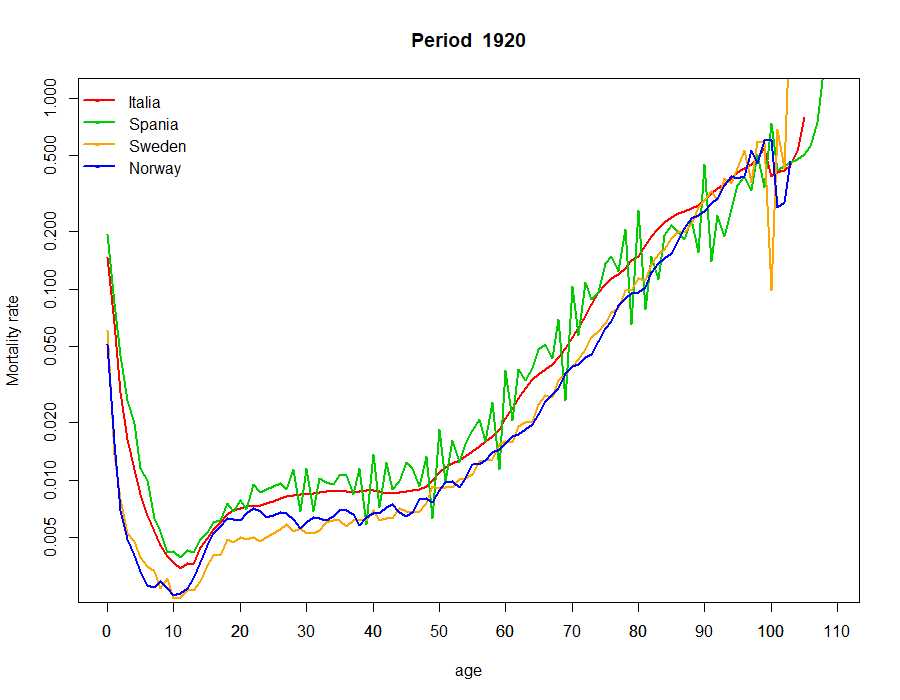
\includegraphics[width=0.8\linewidth]{figures/periodMortalityRate_allCountries1920.png}
              \caption{Period mortality rate for 1920 for all countries.}
              \label{fig:Period mortalityRate 1920}
            \end{figure} 
            
Spain (plotted in green on the figures)  has the highest mortality in 1920 and 1950, followed by Italy. Figures (\ref{fig:Period mortalityRate 1920} and \ref{fig:Period mortalityRate 1950})  
Sweden and Norway have the lowest mortality and their plots almost overlap during the period 1920.
We also observe a high variation of mortality in Spain during that period.               
            
           \begin{figure}[b]
             \centering
              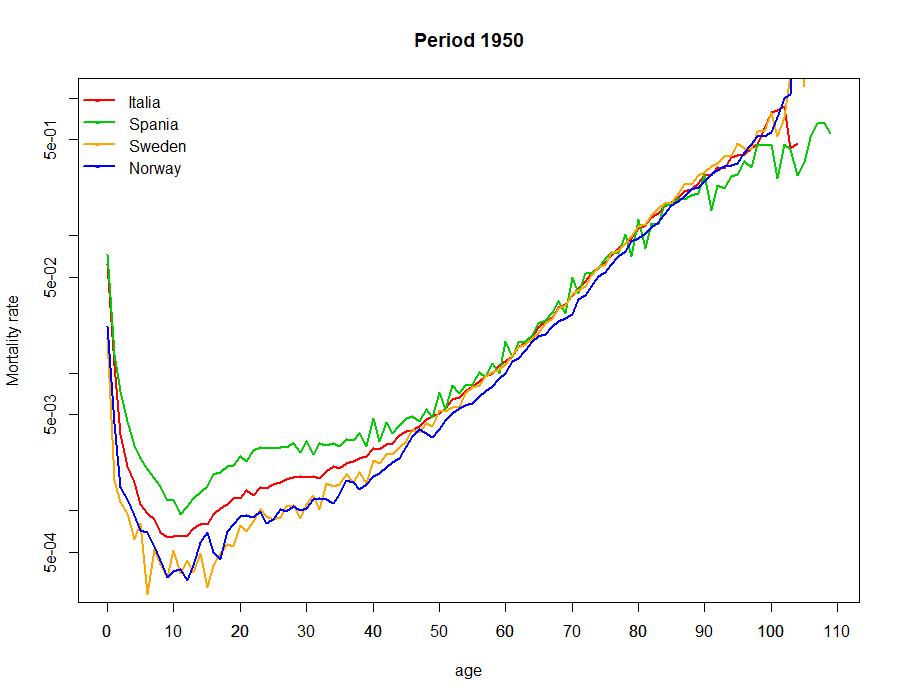
\includegraphics[width=0.8\linewidth]{figures/periodMortalityRate_allCountries1950.png}
              \caption{Period mortality rate for 1950 for all countries.}
              \label{fig:Period mortalityRate 1950}
            \end{figure} 
In the ages 0-55 years there is a gap between the four countries, but after that we observe that Italy and Spain catch up Sweden and Norway, having almost the same mortality. 
Approaching the age 80, we can see on figures \ref{fig:Period mortalityRate 1920} and \ref{fig:Period mortalityRate 1950} that Spain has the lowest mortality rate in 1920 and 1950.           
            
           \begin{figure}[t]
             \centering
              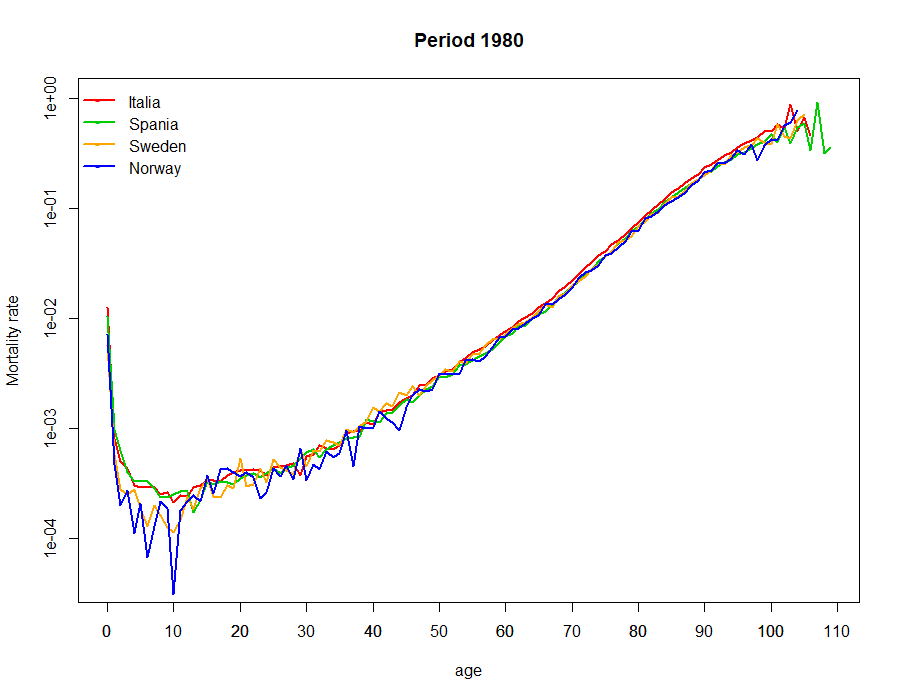
\includegraphics[width=0.8\linewidth]{figures/periodMortalityRate_allCountries1980.png}
              \caption{Period mortality rate for all countries.}
              \label{fig:Period mortalityRate 1980}
            \end{figure} 
            
Figure \ref{fig:Period mortalityRate 1980} shows that during the calendar year 1980  the mortality is very low for all the four countries, Norway (plotted in blue) has the lowest mortality and reaches the lowest level at age 10 on figure \ref{fig:Period mortalityRate 1980}. 

          \begin{figure}[tbh]
             \centering
              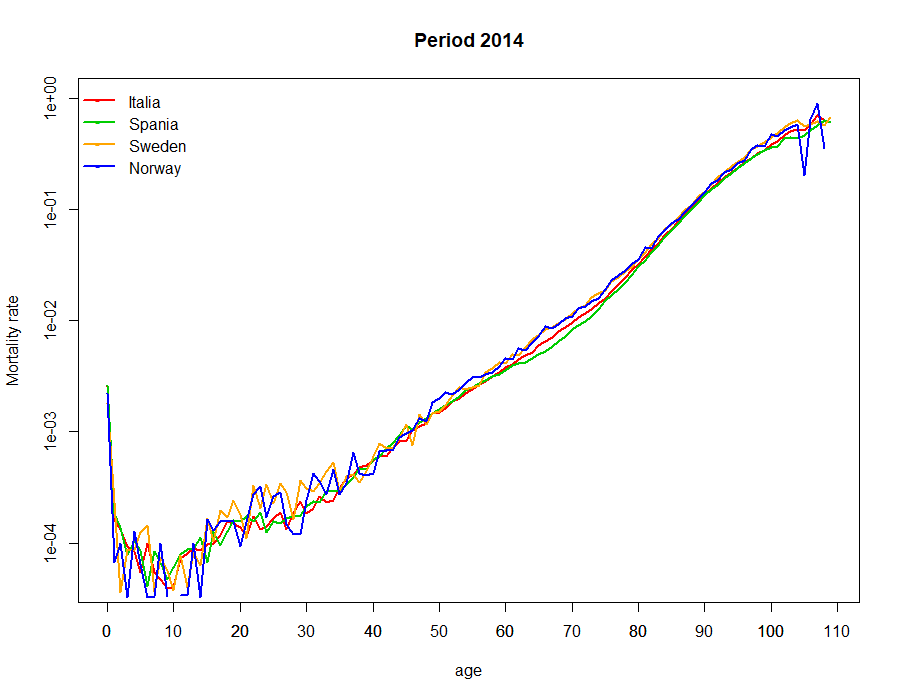
\includegraphics[width=0.8\linewidth]{figures/periodMortalityRate_allCountries2014.png}
              \caption{Period mortality rate for 2014 for all countries.}
              \label{fig:Period mortalityRate 2014}
            \end{figure} 
            
Figure \ref{fig:Period mortalityRate 2014} shows that there is no major difference of mortality between the four countries during the period 2014. 
We observe small jumps between ages 0-40 years for all four countries.
This is due to the use of logarithmic scale on the y-axis and a very low mortality for the low ages.
We observe here that the mortality in Spain and Italy is slightly lower than the mortality in Sweden and Norway around the age 45 and upward.

We can conclude that the trend over the years remains almost the same for Sweden and Norway on one side and for Spain and Italy on the other side.
The mortality in the earlier period was higher in Spain and Italy than in Sweden and Norway, but from the 80s as figure  \ref{fig:Period mortalityRate 1980} illustrates, the gap has gradually reduced as Spain and Italy have surpassed Sweden and Norway as we can observe in figure \ref{fig:Period mortalityRate 2014}. 




\subsection{Period life expectancy}            
 
The life expectancy for the period data are based on the period mortality as we have shown in the figures \ref{fig:Period mortalityRate 1920} to figure \ref{fig:Period mortalityRate 2014} for the years 1920, 1950, 1980 and 2014.            
            \begin{figure}[t]
             \centering
              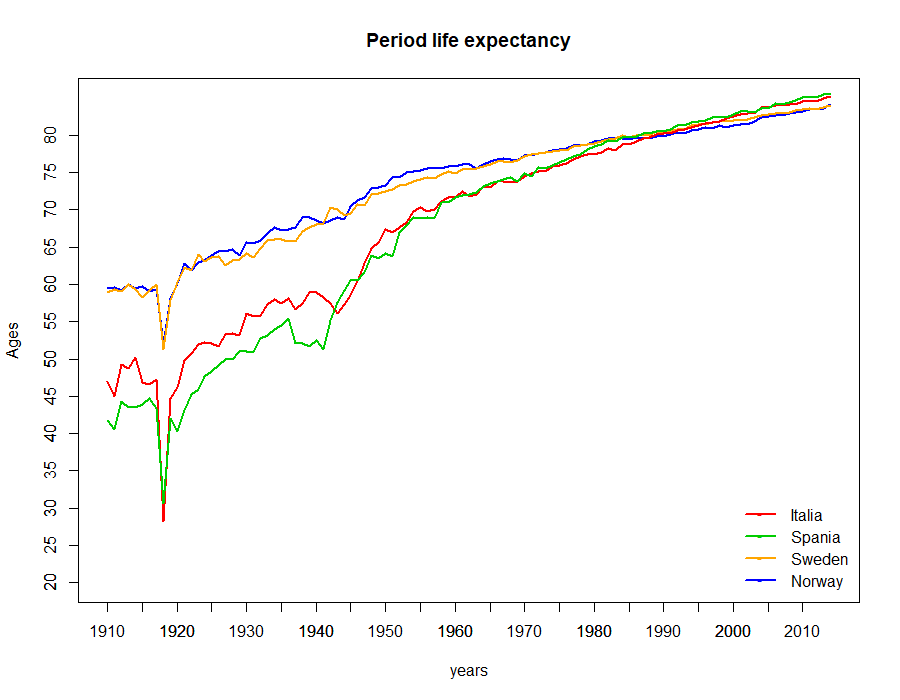
\includegraphics[width=0.8\linewidth]{figures/periodLifeExpectancy_allCountries3.png}
              \caption{Period life expectancy for all the countries.}
              \label{fig:periodLifeExpect all}
            \end{figure}    
            
Figure \ref{fig:periodLifeExpect all} shows the period life expectancy at birth for Italy, Spain, Sweden and Norway from the calendar year 1910 to the calendar year 2014.
We observe a sudden decrease of life expectancy  for all the four countries around the period year 1918. 
This sudden decrease could be the result of the influenza pandemic of 1918-1919 also known as the Spanish flu.
The outbreak of this influenza virus, spread with astonishing speed around the world, killing millions of people.
That may be why the effect is visible in all the four countries.
The plots show that during that period Italy and Spain had the lowest life expectancy around 26 and 28 years respectively, while during the same period Sweden and Norway had about the same life expectancy around 52 years.
Between the two groups we can notice a very big difference of life expectancy, about 24 years.
We also observe a little drop in life expectancy around the calendar years 1938 and 1943 in Spain and Italy respectively, but this time Sweden and Norway remain stable. 
This is probably the result of the Spanish civil war and the world war II.
Apart from the irregular pattern observed in 1918 for all the four countries and during 1938-1943 for Spain and Italy, we observe an increasing trend in life expectancy for all the four countries.
The gap between the two groups, Sweden and Norway on one side and Spain and Italy on the other keeps decreasing over time.
In the latter four decades of the century, life expectancy improvements resulted from mortality reductions for younger ages and those over age 45.
Notice that life expectancy in the 80s is almost the same for all the four countries and beyond that we can observe that women in Spain and Italy seem to have a longer life expectancy than women in Sweden and Norway. 
For the period 2014 the life expectancy at birth for women in Spain was 85.62 years, 85.17 years in Italy, 84.09 years in Norway and 84.05 years in Sweden. Thus, women in the Mediterranean are expected to live about one and a half year longer than those in Scandinavia. 
Progress in the treatment of cardiovascular disease and some forms of cancer on the one hand, and on the other the progress made in the prevention of certain "man-made" diseases, such at alcoholism, smoking or accidents, have made the life expectancy increase  rapidly in the Mediterranean. (\cite{VM04})

 
 
 
\section{Cohort data} 
 
In order to have complete information on a cohort, it has to be observed from birth to extinction (i.e., the date by which all cohort members are assumed to have died).
However, for our data this is only the case for the cohorts born around 1910.
For the younger cohorts, we only have mortality information up to the age of the cohort in 2014.
% kommenter eventuelt hvilke aldere du har informasjon om fra 1910 kohort ( fig. 4.6)    


\subsection{Cohort mortality}            
            
            
              
          \begin{figure}[tbh]
             \centering
              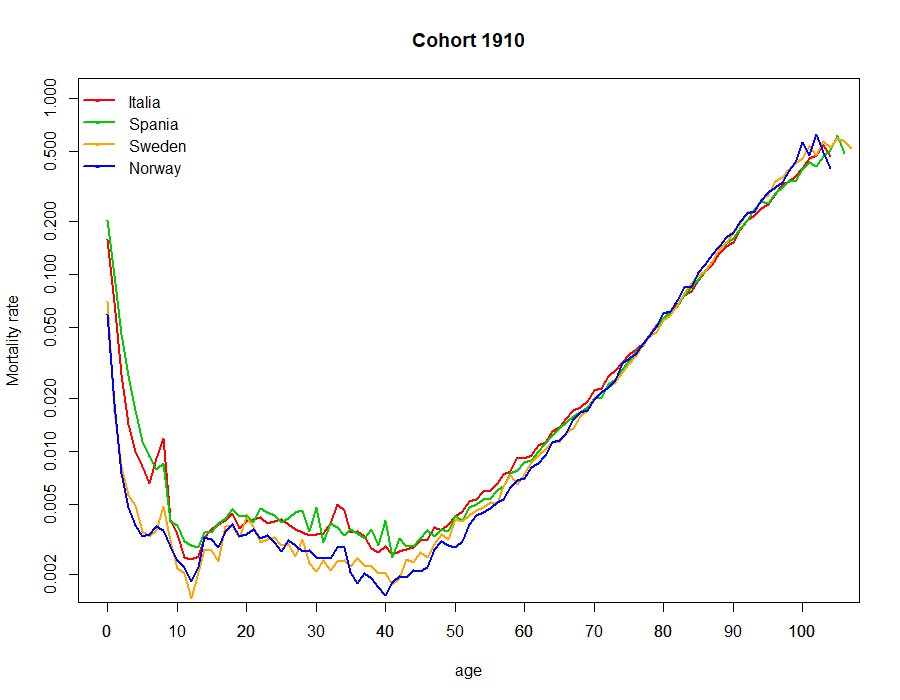
\includegraphics[width=0.8\linewidth]{figures/cohortMortalityRate_allCountries1910.png}
              \caption{Cohort mortality rate for cohort born in 1910 for all countries.}
              \label{fig:CohortMortality 1910}
            \end{figure} 
  
%As observed in the period data, there is a higher concentration of mortality at ages 0-5 years and ages 80-110 years. On Figures . 
Figure \ref{fig:CohortMortality 1910} shows the mortality rates of the cohorts born in 1910.
We can observe that mortality gradually decrease for all the countries and reaches a minimum level around 12 years.
Between the ages 0-8, we can see that Spain has the highest mortality, followed by Italy while the mortality in Sweden and Norway are almost the same.
We observe a reduction in mortality from the age 15 until the age 50 for all those countries.
This is most likely caused by increased living standard.
%In that age group, we see some small jumps but with very little variation of mortality.
From age 50 mortality starts to increase gradually and the gap between the countries decreases.
On figure \ref{fig:CohortMortality 1910} we can observed that the mortality from age 70 is almost the same in all the four countries.
            
            
              
          \begin{figure}[tbh]
             \centering
              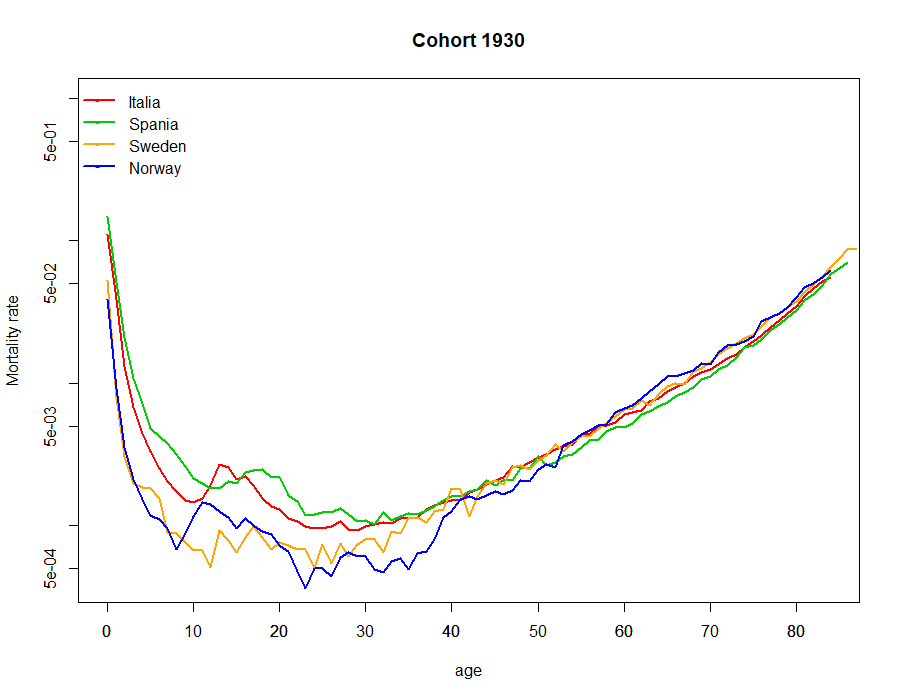
\includegraphics[width=0.8\linewidth]{figures/cohortMortalityRate_allCountries1930.png}
              \caption{Cohort  mortality rate for cohort born in 1930 for all countries.}
              \label{fig:CohortMortality 1930}
            \end{figure} 
The mortality for the cohort born in 1930 is shown in figure \ref{fig:CohortMortality 1930}.
We can observe that there is a clear difference of mortality between the four countries from the age 5 years until the age 40 years.
This is contrary to the cohort 1910 where the mortality in Sweden overlaps with Norway and the mortality in Spain with the one in Italy.        
Spain and Italy have the highest mortality up to ages 50-60 years, but it is the contrary for older ages.            
            
              
          \begin{figure}[tbh]
             \centering
              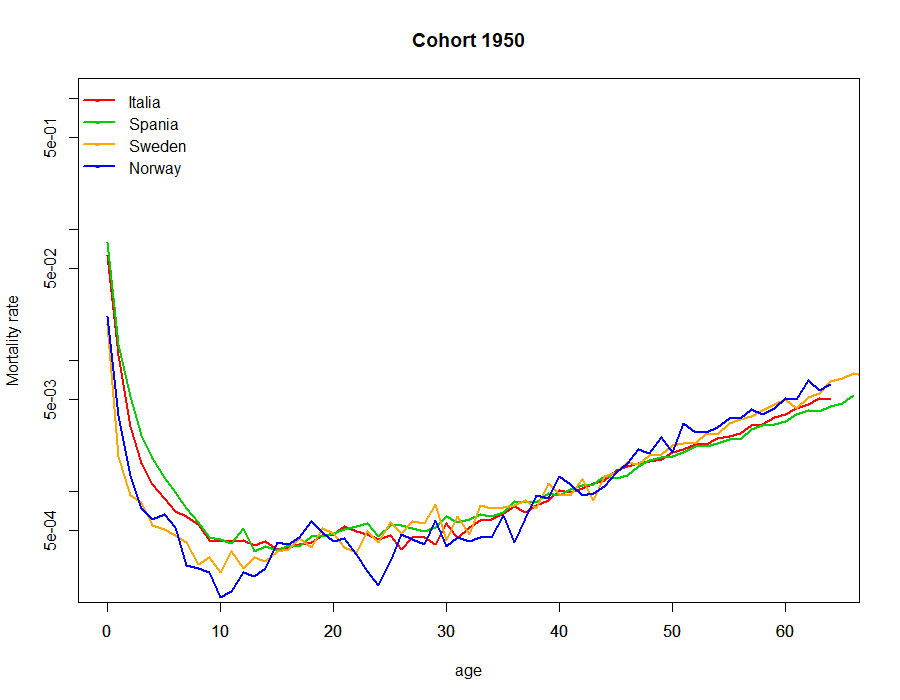
\includegraphics[width=0.8\linewidth]{figures/cohortMortalityRate_allCountries1950.png}
              \caption{Cohort mortality rate for cohort born in 1950 for all countries.}
              \label{fig:CohortMortality 1950}
            \end{figure} 
            
Figure \ref{fig:CohortMortality 1950} shows that Norway (blue line) has the lowest level of mortality for the cohort 1950 with the minimum around the ages 10 years and 24 years.
We also observe an unstable development in the Norwegian mortality with a lot of jumps from age 10 years to age 50 years.
Her also the unstable development could be due to the very low mortality and the logarithmic scale.
We also have low mortality in Sweden and Norway up to around 50 years, but we observe the contrary beyond that.

            
              
          \begin{figure}[tbh]
             \centering
              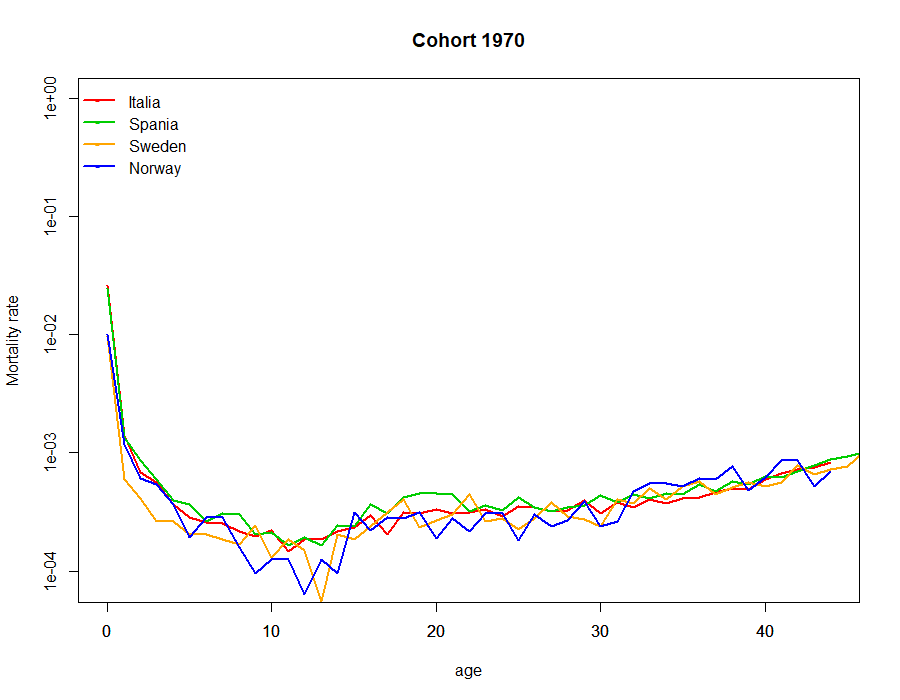
\includegraphics[width=0.8\linewidth]{figures/cohortMortalityRate_allCountries1970.png}
              \caption{Cohort mortality rate for cohort born in 1970 for all countries.}
              \label{fig:CohortMortality 1970}
            \end{figure} 
            
          
 Figure \ref{fig:CohortMortality 1970} shows a decrease of the mortality for all the countries, reaching minimum mortality at age 12 years for Norway and 14 years for Sweden.
 Sweden and Norway show an increase from the minimum to a plateau for young adults.
 From age 15 to age 45, we can observe a quite stable and low variation of mortality for all the countries, forming a plateau.
 
We can conclude that the gap of mortality is bigger in the earlier age groups for cohort data than in period data. 
We also observed a slower decrease of mortality among the younger in the cohort data than in the period data.
In the case of cohort, we can observe a smaller concentration of mortality in the earlier ages than in the older ages group. 
While Sweden and Norway have the lowest mortality in the younger ages, we observe the contrary for the aged.

       
       
       


% Si je dois explique ma these de Master : There exist two types of life table, period life table and cohort life table. In Period life table, death rates refer to mortality experience during only one calendar year, for person born in many different years. In reality, people do not behave that way: They are born in only one year, and they live their lives during many calendar years.In cohort life table we have age specific death rates for persons born one particular year as they age (many different calendar years). Cohort life table may lead to different conclusion than period life tables about life expectancy.
            
            
\subsection{Expected number of years lost for cohorts}         


In this section, we want to look at the expected number of year lost for cohort data.     
In order to compute the cohort life expectancy accurately, we need the complete mortality history of a cohort, and this is only possible for older cohorts that were born more than 100 years ago. For younger cohorts, we are not able to compute the cohort life expectancy.
In this thesis, we therefore suggest that one may instead consider the expected number of years lost for a cohort up to a given age. (\cite{A13}) 
Then, by computing the expected number of years lost for a number of cohorts, one will obtain a good picture of the longevity in a country that is only based on the available data
for the cohorts.



              \begin{figure}[tbh]
             \centering
              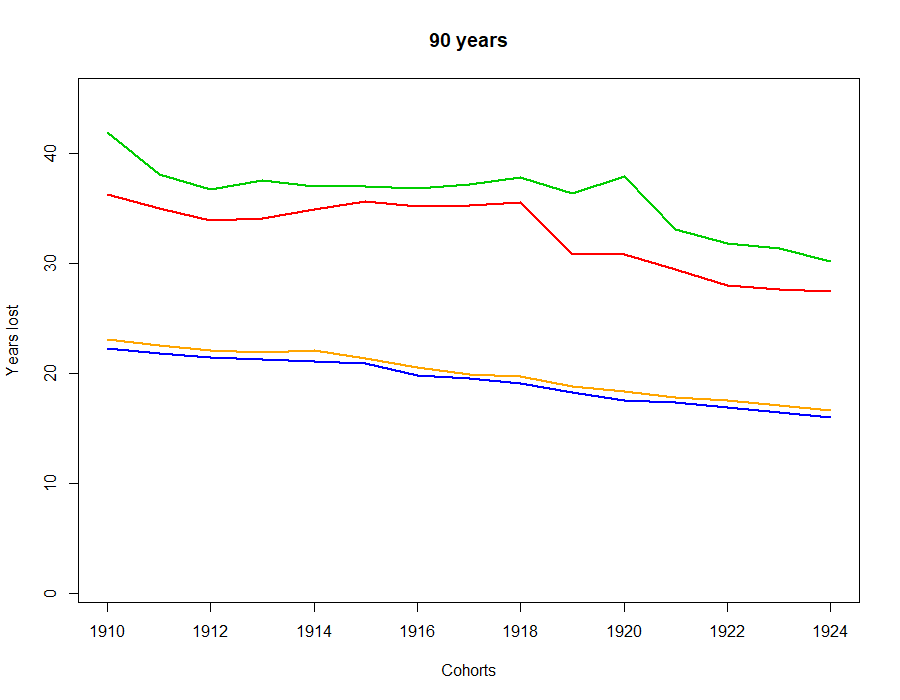
\includegraphics[width=0.8\linewidth]{figures/antal_tapteAA_age90.png}
              \caption{Number of years lost. Here we fix the age and consider the expected number of years lost as a function of cohort.}
              \label{fig:Number years lost max years90}
              \end{figure}          
Figures \ref{fig:Number years lost max years90} - \ref{fig:Number years lost max years40 } show the expected number of years lost up to the ages 90, 80, 70, 60, 50 and 40 in Spain, Italy, Sweden and Norway.
The scales on the y-axis are adjusted in order to have a better visualization of the four countries.
The expected number of years lost up to 90 years, figure \ref{fig:Number years lost max years90}, shows that Spanish (green plot) and Italian (red plot) women have lost more years of life than Swedish (orange plot) or Norwegian (blue plot).
We can observe some little variations in Italy and Spain for the cohort 1919 and 1920 respectively.
 
            
            
                            
              \begin{figure}[tbh]
             \centering
              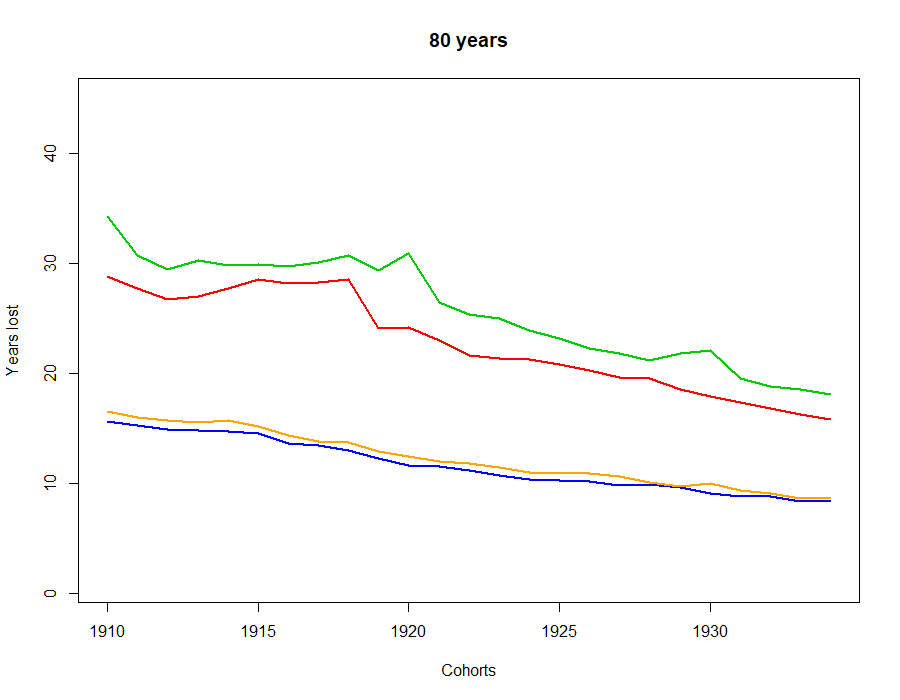
\includegraphics[width=0.8\linewidth]{figures/antal_tapteAA_age80.png}
              \caption{Number of years lost. Here we fix the age and consider the expected number of years lost as a function of cohort.}
              \label{fig:Number years lost max years80}
            \end{figure}          
                    

The expected number of years lost up to age 80 in figure  \ref{fig:Number years lost max years80}, have almost the same trend as in figure \ref{fig:Number years lost max years90}.
Sweden and Norway remain close to each other but the gap between them and Spain and Italy is still very high.
Here also we observe a little jump around the cohort 1930 but only in Spain.
            
            
            
                              
              \begin{figure}[tbh]
             \centering
              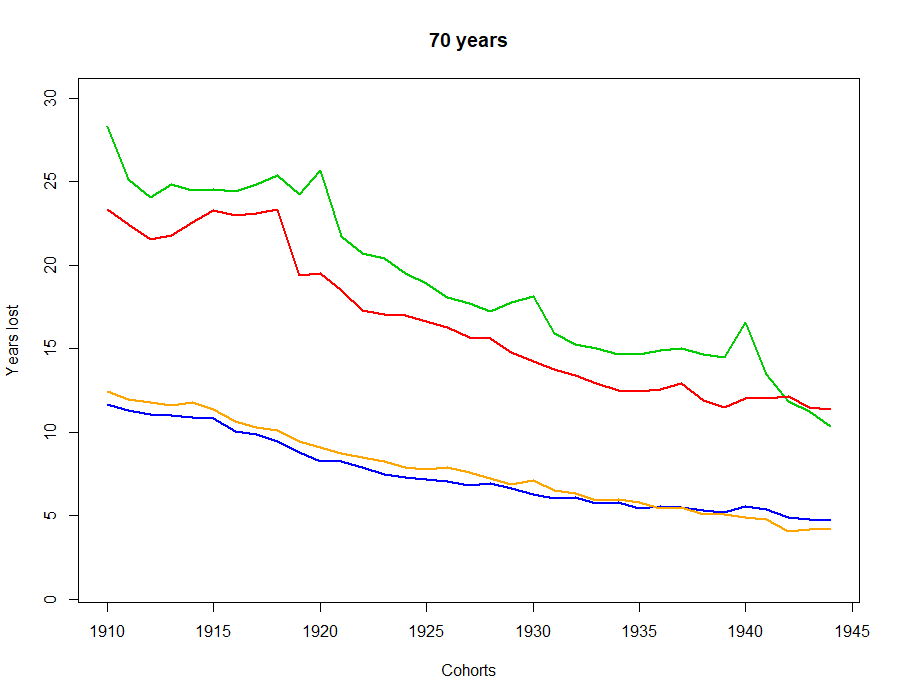
\includegraphics[width=0.8\linewidth]{figures/antal_tapteAA_age70.png}
              \caption{Number of years lost. Here we fix the age and consider the expected number of years lost as a function of cohort.}
              \label{fig:Number years lost max years70 }
            \end{figure}          
 
                  
Figure \ref{fig:Number years lost max years70 } shows the expected number of years lost up to age 70. 
We observe that the gap between all the countries is larger for 70 years than for 80 years.
Women in Sweden and Norway lose fewer years than women in Spain and Italy.

            
            
            
                               
              \begin{figure}[tbh]
             \centering
              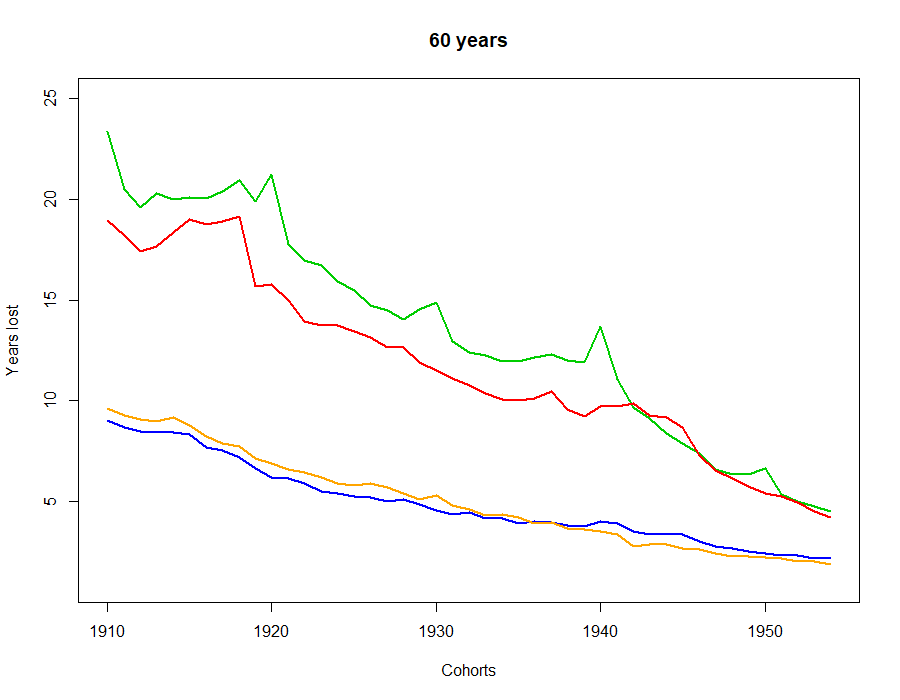
\includegraphics[width=0.8\linewidth]{figures/antal_tapteAA_age60.png}
              \caption{Number of years lost. Here we fix the age and consider the expected number of years lost as a function of cohort.}
              \label{fig:Number years lost max years60 }
            \end{figure}          
                 
            
            
            
            
                                 
              \begin{figure}[tbh]
             \centering
              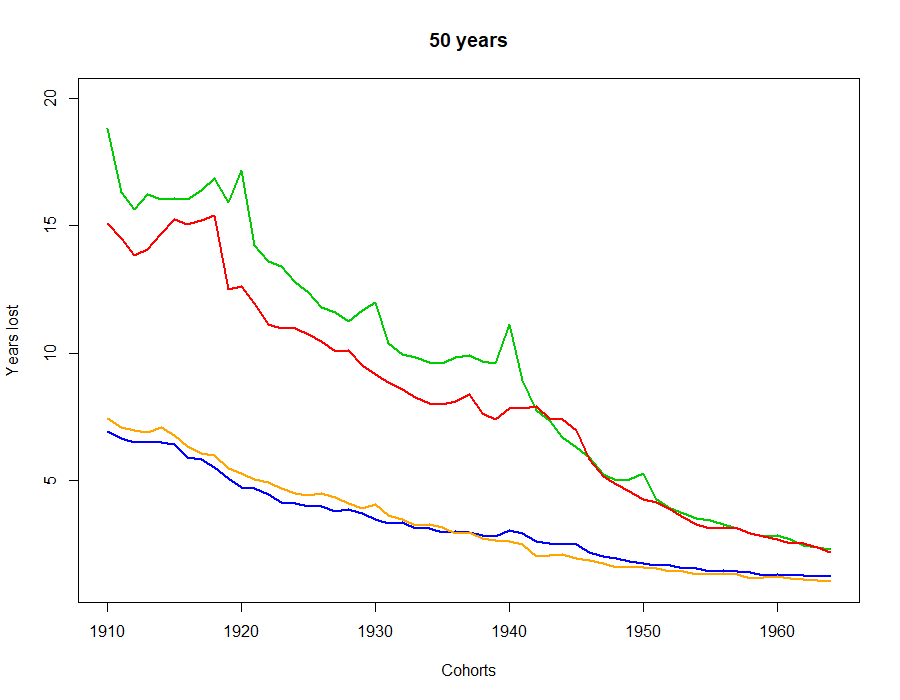
\includegraphics[width=0.8\linewidth]{figures/antal_tapteAA_age50.png}
              \caption{Number of years lost. Here we fix the age and consider the expected number of years lost as a function of cohort.}
              \label{fig:Number years lost max years50 }
            \end{figure}          
               
On figures \ref{fig:Number years lost max years50 } and \ref{fig:Number years lost max years60 }, we can observe that the expected number of years lost decreases with time for all the cohorts. 
But it seems to decrease faster in Spain and Italy than in Sweden and Norway.
We can also observe an increase of variation for all the countries.
            
            
            
                                    
              \begin{figure}[tbh]
             \centering
              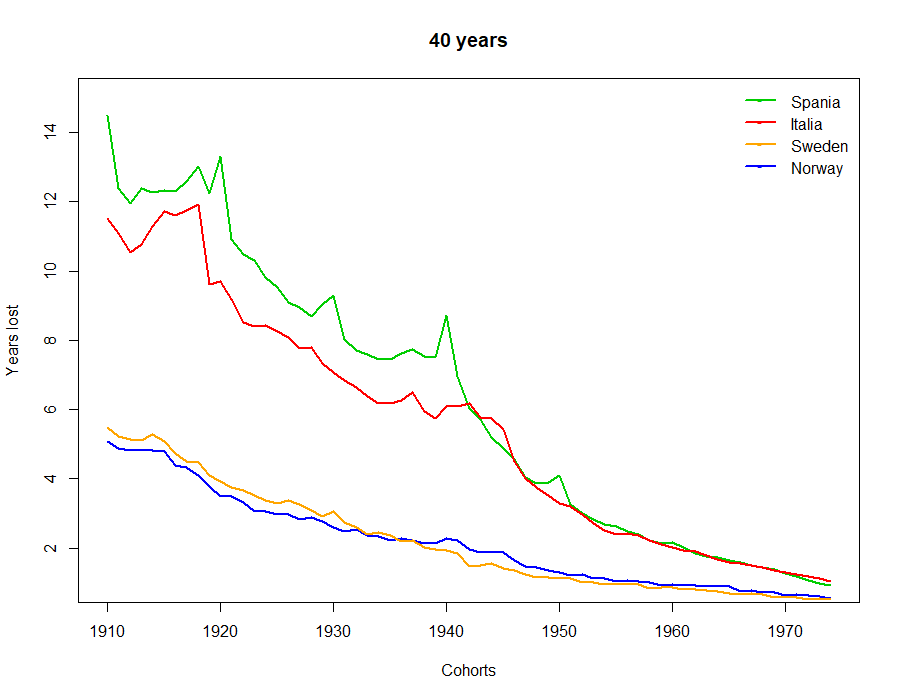
\includegraphics[width=0.8\linewidth]{figures/antal_tapteAA_age40.png}
              \caption{Number of years lost. Here we fix the age and consider the expected number of years lost as a function of cohort.}
              \label{fig:Number years lost max years40 }
            \end{figure}          

Figure \ref{fig:Number years lost max years40 }  shows the plots of the expected number of years lost up to the age 50 for the four countries. 
Around the 70s we can see that Spain and Italy have gained about 12 and 14 years respectively but Sweden and Norway still have the lowest expected number of years lost.
            

            
                        
              \begin{figure}[tbh]
             \centering
              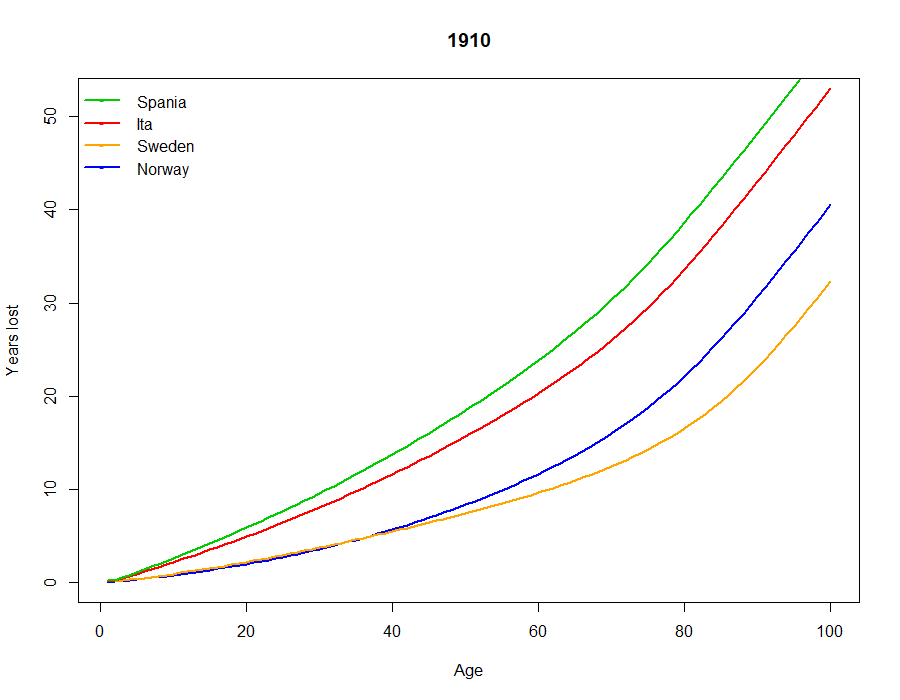
\includegraphics[width=0.8\linewidth]{figures/antal_tapteAs_functionCohort_AllCountries1910.png}
              \caption{Number of years lost. Here we fix the cohort and look at the expected number of years lost as a function of age.}
              \label{fig:Number of years lost 1910}
            \end{figure}   
             
 Figures \ref{fig:Number of years lost 1910} - \ref{fig:Number of years lost 1970} show the expected number of years lost but this time we fix the cohort and look at the expected number of years lost as a function of age.  
 The lines on these figures slope upwards to the right.
 As the cohort increases, the expected number of years lost decreases.

              \begin{figure}[tbh]
             \centering
              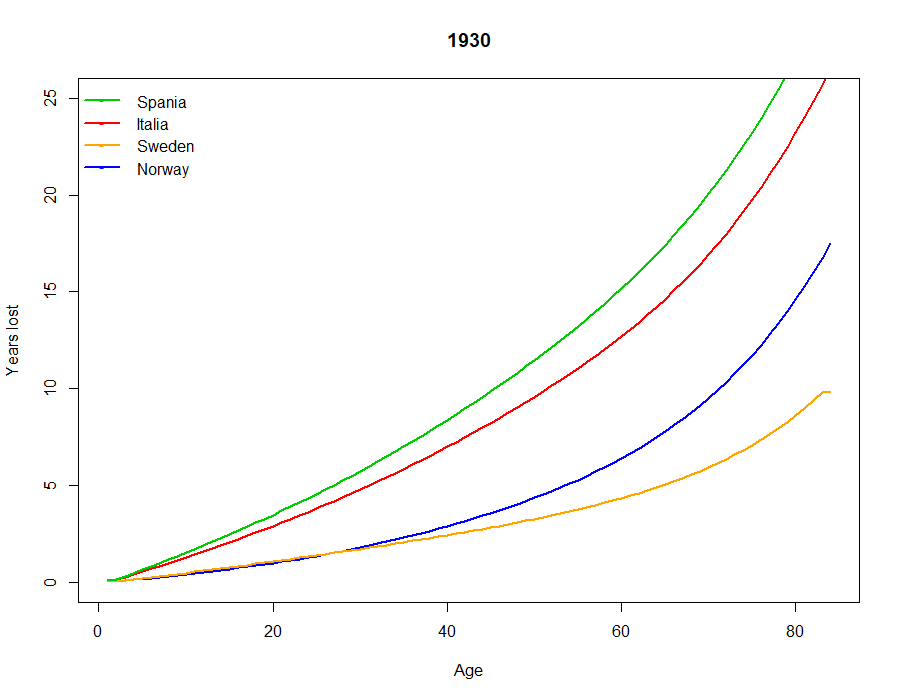
\includegraphics[width=0.8\linewidth]{figures/antal_tapteAs_functionCohort_AllCountries1930.png}
              \caption{Number of years lost. Here we fix the cohort and look at the expected number of years lost as a function of age.}
              \label{fig:Number of years lost 1930}
            \end{figure}   
            
         
                         
              \begin{figure}[tbh]
             \centering
              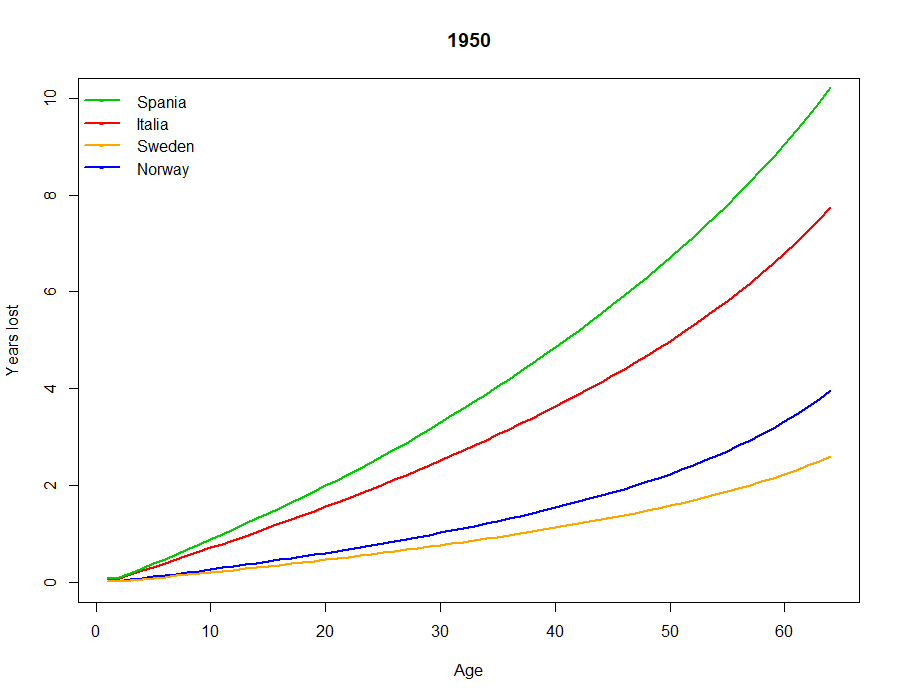
\includegraphics[width=0.8\linewidth]{figures/antal_tapteAs_functionCohort_AllCountries1950.png}
              \caption{Number of years lost. Here we fix the cohort and look at the expected number of years lost as a function of age.}
              \label{fig:Number of years lost 1950}
            \end{figure}   
            
            
            
         
                         
              \begin{figure}[tbh]
             \centering
              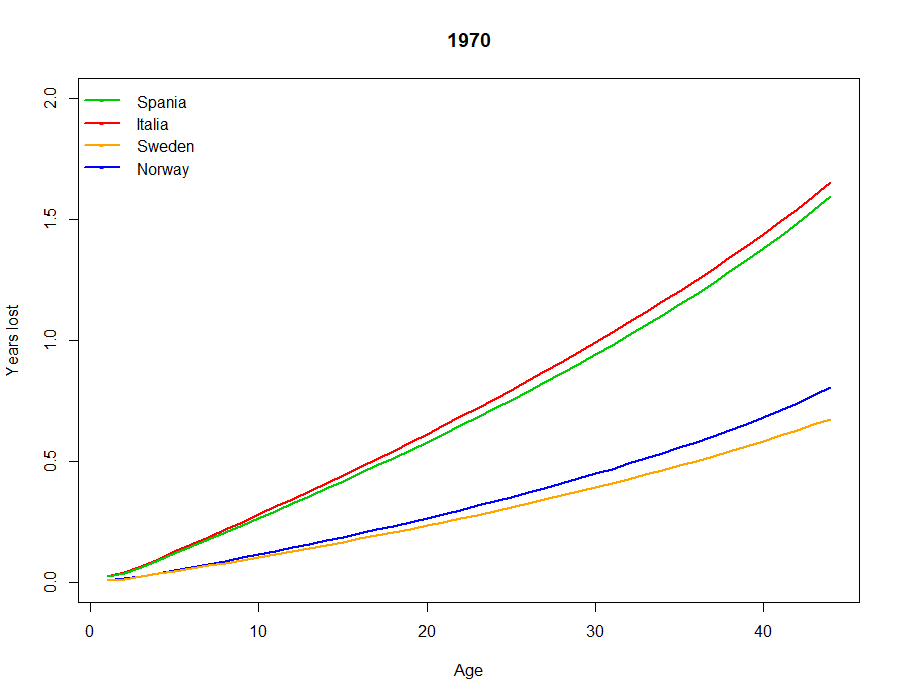
\includegraphics[width=0.8\linewidth]{figures/antal_tapteAs_functionCohort_AllCountries1970.png}
              \caption{Number of years lost. Here we fix the cohort and look at the expected number of years lost as a function of age.}
              \label{fig:Number of years lost 1970}
            \end{figure}   
            
The gap between Spain and Italy on one side and Sweden and Norway on the other side has been considerably reduced as we can observe in figure \ref{fig:Number of years lost 1970}. 
But for all cohorts and ages, women in Spain and Italy may expect to loose more years than women in Sweden and Norway.

            
 \section{Summary of the chapter } 
 
The plots of our estimates suggest that during the 20th century, mortality rates have declined quite rapidly in the Mediterranean and the Scandinavian countries.
We saw that mortality was highly concentrated among the younger and the aged in all those countries.
Despite the fact that mortality was very high for all those countries, there was a huge gap between the two regions and that gap has continuously decreased over time.
The steady reduction of mortality over the years leads to an improvement of live expectancy.
The period data suggested that from the first decade of the 20th century to the 80s, women lived longer in Sweden and Norway than in Spain and Italy. 
But after the 80s we observed that women in Spain and Italy seemed to have caught up and even passed Sweden and Norway, having the higher life expectancy.
But looking at the cohort data we can see a different picture.
In fact the figures of the expected number of year lost tells us that women in Norway and Sweden are still expected to lose fewer years than those in Spain and Italy. 
In the next chapters we will look at a possible explanation of the conflicting results for period and cohort data.







